\documentclass[11pt]{article}
\usepackage[margin=1in]{geometry}
\usepackage{amsmath, amssymb, amsthm, esint}
\usepackage{fancyhdr}
\usepackage{tikz, tikz-3dplot}
% \usepackage{hyperref}
\usepackage{enumitem}
\usepackage{float}
\usepackage{cancel}

\pagestyle{fancy}
\fancyhf{}
\setlength{\headheight}{14pt}
\lhead{Miscellany}
\cfoot{\thepage}

\begin{document}
\begin{center}
    \tableofcontents
\end{center}
\setcounter{page}{1}
\newpage
\section{An Eigenvalue Approach to the Fibonacci Sequence}
\subsection{Introduction}
The Fibonacci Sequence is a one of the most famous sequence in mathematics. It is defined by the recurrence relation:
\[
    \begin{cases}
        \,F_n=F_{n-1}+F_{n-2},\text{ for }n \geq 2\\[.5em]
        \,F_0=F_1=1
    \end{cases}    
\]
Each term is the sum of the two preceeding terms: $1,1,2,3,5,8\dots$
\subsection{Matrix Representation of the Fibonacci Sequence}
Let 
\[
    x_0=\begin{bmatrix}
        F_1\\F_0
    \end{bmatrix}
    \text{, } x_1 =\begin{bmatrix}
        F_2\\F_1
    \end{bmatrix}
    \text{, and }A=\begin{bmatrix}
        1&1\\1&0
    \end{bmatrix}
\]
By repeatedly applying the matrix $A$, we can express each term of the sequence as a power of $A$ acting on $x_0$:
\begin{align*}
    &x_1 = A x_0, \\
    &x_2 = A x_1 = A (A x_0) = A^2 x_0\\
    &\Rightarrow \,\, x_n = A^nx_0
\end{align*}
\subsection{General Eigenvalue Method}
For a Matrix $A \in \mathbb{R}^{2\times 2}$ with two distinct eigenvalues and two corresponding eigenvectors, we know that any vector is a linear combonation of $v_1$ and $v_2$, i.e.
\begin{align*}
    \begin{cases}
        Av_1=\lambda_1 v_1\\
        Av_2=\lambda_2 v_2
    \end{cases}\text{, and }
    v=av_1+bv_2
\end{align*}
Applying $A$ repeatedly to $v$ and using the eigenvalue property gives, 
\begin{align*}
    Av &=a\lambda_1 v_1+b\lambda_2 v_2, \\
    A^2v &= a\lambda_1^2 v_1+b\lambda_2^2 v_2, \\
    &\quad\vdots \\
    \Rightarrow\, A^nv&=a\lambda_1^n v_1+b\lambda_2^n v_2.
\end{align*}
\subsection{Application to the Fibonacci Matrix}
Let us now consider the Fibonacci matrix
\[
    A = \begin{bmatrix} 1 & 1 \\ 1 & 0 \end{bmatrix}.
\]
Its eivenvalues are given by the \textbf{characteristic eqaution}
\[
    \det(\lambda I-A)=\begin{vmatrix}
        \lambda-1 & -1\\-1 & \lambda
    \end{vmatrix}=0 \Rightarrow \boxed{\lambda^2 - \lambda - 1 = 0}
\]
, and a quick computation yields $\displaystyle\lambda = \varphi \,_\lor -\frac{1}{\varphi}$.\\
\subsubsection*{Notice that this is exactly the same as the equation obtained from assuming $F_n = \lambda^n$ in the Fibonacci recurrence:}
\[
    F_n = F_{n-1} + F_{n-2} \Leftrightarrow \lambda^n  = \lambda^{n-1} + \lambda^{n-2} \Rightarrow  \boxed{\lambda^2  = \lambda + 1}
\]
\subsection{Deriving the Closed Form}
We can now express $x_n = A^n x_0$ explicitly in terms of $\lambda_1$ and $\lambda_2$. Let us consider
\[
    F_n=p\cdot\varphi^n + q\cdot(-\frac{1}{\varphi})^n
\]
By initial contidion $F_0=F_1=1$, 
\[
    \begin{cases}
        \displaystyle
        \,p+q=1\\
        \displaystyle
        \,p\cdot\varphi + q\cdot (-\frac{1}{\varphi}) = 1
    \end{cases}
    \Rightarrow
    \begin{cases}
        \displaystyle
        \,p=\frac{1}{\sqrt{5}}\varphi\\
        \displaystyle
        \,q=-\frac{1}{\sqrt{5}}\frac{1}{\varphi}
    \end{cases}
\]
Thus, 
\[
    F_n = \frac{1}{\sqrt{5}}\left[\varphi^{n+1} - (-\frac{1}{\varphi})^{n+1}\right] _\#
\]
\subsection{Similar Problems}
\subsubsection{Non-linear Recurrence Equation}
Given $a_n=3a_{n-1}+2$  and $a_1 = 2,\,a_2 = 8$. Find the general formula for $a_n$. 
\subsubsection*{Solution}
We start by  homogeneous linear equation
\[
    a_n=3a_{n-1}\Rightarrow x^2=3x
\]
Quick calculation gives $\displaystyle x=0 \,_\lor \,3$, then we assume the general formula in eigenvalue approach plus a displacement $r$.
\[
    a_n=p\cdot 3^n + q\cdot 0^n + r
\]
By initial condition $a_1 = 2,\, a_2 = 8$
\[
    \begin{cases}
        \displaystyle
        \,3p+r=2\\
        \displaystyle
        \,9p+r=8\\
    \end{cases}
    \Rightarrow
    \begin{cases}
        \displaystyle
        \,p=1\\
        \displaystyle
        \,q=-1\\
    \end{cases}
\]
Thus the general formula for $a_n$ is 
\[
    a_n = 3^n - 1 _\#
\]
\subsubsection{Five-Color Planar Graph Coloring}
\subsubsection*{Solution}



\section{Zero Forcing Game}
\subsection{The game itself}
The set of linear equation 
$\begin{cases}
    ax+by=0\\
    a\neq 0, y= 0
\end{cases}$ implies that $x=0$. We can generalize these condition to: 
\[
    \begin{cases}
        \displaystyle
        \,a_1x_1+a_2x_2+\dots+a_nx_n\\
        \displaystyle
        \,a_1 \neq 0 \, \& \, x_i = 0 \text{ for } i \geq 2
    \end{cases}
\]
\subsection{Trun into Graph}
\vspace{10pt}
\begin{minipage}{.3\textwidth}
    \centering
    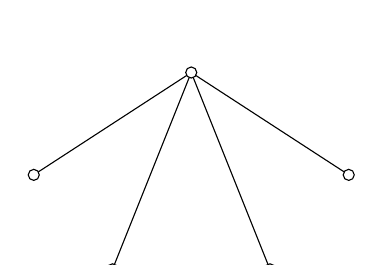
\begin{tikzpicture}
        % \tikzset{point/.style={circle,draw,fill=white,inner sep=1.5pt}}
        % \node[point] at (A) {};
        \coordinate (A) at (-2, .7);
        \coordinate (B) at (-1, -.5) ;
        \coordinate (C) at (1, -.5);
        \coordinate (D) at (2, .7);
        \coordinate (E) at (0, 2);

        \draw[black] (A)--(E);
        \draw[black] (B)--(E);
        \draw[black] (C)--(E);
        \draw[black] (D)--(E);

        \filldraw[fill=white,draw=black] (A) circle (2pt);
        \filldraw[fill=white,draw=black] (B) circle (2pt);
        \filldraw[fill=white,draw=black] (C) circle (2pt);
        \filldraw[fill=white,draw=black] (D) circle (2pt);
        \filldraw[fill=white,draw=black] (E) circle (2pt);
    \end{tikzpicture}
\end{minipage}
\hfill
\begin{minipage}{.6\textwidth}
    \vspace{0pt}
    \textbf{Coloring Rules}
    \begin{enumerate}
        \item If a black vertex has exactly one white neighbor, then the white neighbor is forced to be black.
        \item Repeat until no more changes occur.
    \end{enumerate}
\end{minipage}
\subsection{The Adjacency Matrix}
Let $G = (V,E)$ with $V = \{v_1, v_2, \dots, v_n\}$. The \textbf{Adjacency Matrix} $A=(a_{ij})$ of $G$ is
\[
    a_{ij} = 
    \begin{cases}
        \displaystyle
        \,1 & \text{if } \{v_i,v_j\}\in E,\\
        \displaystyle
        \,0 & \text{otherwise}.
    \end{cases}
\]
e.g. For a path graph $G \in P_n$, the adjacency matrix is 
\newline
\begin{minipage}{\textwidth}
    \centering
    \begin{minipage}[][70pt][c]{.3\textwidth}
        $P_4\,$ 
        \centering
        \begin{tikzpicture}[scale=.6]
            \draw (-3, 0) --(3,0);

            \filldraw[fill=white, draw=black] (-3, 0) circle (2pt);
            \filldraw[fill=white, draw=black] (-1, 0) circle (2pt);
            \filldraw[fill=white, draw=black] (1, 0) circle (2pt);
            \filldraw[fill=white, draw=black] (3, 0) circle (2pt);
        \end{tikzpicture}
    \end{minipage}
    \begin{minipage}[m][70pt][c]{.2\textwidth}
    \vfill
    \[
        \Rightarrow
        \begin{bmatrix}
            0 & 1 & 0 & 0\\
            1 & 0 & 1 & 0\\
            0 & 1 & 0 & 1\\
            0 & 0 & 1 & 0\\
        \end{bmatrix}
    \]
    \vfill
    \end{minipage}
\end{minipage}
\subsection{Appendix}
\subsubsection{Eigenvalue of path graph $\boldsymbol{P_n}$ }
Let $p_n$ denote the characteristic polynomial of path $P_n$
The recurrence formula is given by
\begin{align*}
    \begin{cases}
        p_{n+2} = \lambda p_{n+1} + p_n\\
        p_0 = 1, \,p_1 = \lambda
    \end{cases}
    \overset{\text{Ansatz } r^n\,=\,p_n}{\Rightarrow}
    \quad
    &r^2 = \lambda r - 1
\end{align*}
Solving $r^2 = \lambda r - 1$ gives 
\[
    r = \frac{\lambda \pm \sqrt{\lambda^2-4}}{2}
\]
By Gershgorin's Theorem, $|\lambda|\leq 2$\\
Let 
\[
    \lambda = 2\cos\theta \Rightarrow r=\cos\theta \pm i\sin\theta = e^{\pm i\theta}
\]
Therefore,
\[
    p_n(\lambda)=\alpha e^{i\text{n}\theta} + \beta e^{-i\text{n}\theta}
\]
By initial condition $p_0 = 1, \,p_1=\lambda$
\[
    \begin{cases}
        \alpha + \beta = 1\\[.5em]
        \alpha e^{i\theta} + \beta e^{-i\theta}=\lambda=2\cos\theta
    \end{cases}
\]
A quick calculation yields
\[
    \alpha = \frac{e^{i\theta}}{2i\sin\theta},\,\beta = \frac{-e^{-i\theta}}{2i\sin\theta}
\]
Now $\lambda = 2\cos\theta$ and
\[
    \begin{split}
        p_n(\lambda)&=\frac{e^{i\theta}}{2i\sin\theta}\cdot e^{i\text{n}\theta} + \frac{-e^{-i\theta}}{2i\sin\theta}\cdot e^{-i\text{n}\theta}\\[.5em]
        &=\frac{e^{i(\text{n+1})\theta}-e^{-i(\text{n+1})\theta}}{2i\sin\theta}\\[.5em]
        &=\frac{\sin((n+1)\theta)}{\sin\theta}
    \end{split}
\]

\end{document}